\documentclass[10pt]{beamer}

\usetheme{Boadilla}

\usepackage{pgf}
\usepackage[english]{babel}
\usepackage[utf8]{inputenc}
\usepackage{epstopdf}

\usepackage{bm}
%\usepackage[opticals,mathlf,onlytext]{MinionPro}
\usepackage{mathpazo}
\usepackage[euler-digits,euler-hat-accent]{eulervm}

%\setbeamercolor{structure}{fg=Ma}

%\usepackage{times}
%\usepackage[T1]{fontenc}

%\usepackage{graphicx}
%\usepackage{epstopdf}
%\DeclareGraphicsExtensions{.pdf,.eps,.png,.jpg,.mps} 

\title[Defensa de Tesis] %
{Segmentaci\'on de interlocutores a partir de se\~nales de audio utilizando cadenas escondidas de Markov  y t\'ecnicas de selecci\'on autom\'atica de modelos}

%\subtitle{Include Only If Paper Has a Subtitle}

\author[Rafael de Jes\'us Robledo Ju\'arez]%
{Rafael de Jes\'us Robledo Ju\'arez \\
\small{\texttt{rrobledo@cimat.mx}} \\ ~\\
\small{Asesor: Dr. Salvador Ru\'iz Correa}}


\institute[CIMAT] % (optional, but mostly needed)
{
  \pgfuseimage{university-logo} ~ \\
  Centro de Investigaci\'on en Matem\'aticas, Guanajuato \\
  Departamento de Ciencias de la Computación
}

\date[noviembre 2013]
{xx de noviembre del 2013}
\subject{\title}

\pgfdeclareimage[interpolate=true, height=2cm]{university-logo}{logos/logo-big}
\pgfdeclareimage[interpolate=true, height=0.5cm]{department-logo}{logos/logo-trans}
%\logo{\pgfuseimage{department-logo}}
\logo{
	\pgfputat{\pgfxy(-0.3, 0)}{
    %\begin{pgfrotateby}{\pgfdegree{30}}
    %  \pgfbox[center,base]{\pgfuseimage{department-logo}}
    %\end{pgfrotateby}
	}
}

\AtBeginSection[] {
  \begin{frame}
   \frametitle{Contenido}
    \tableofcontents[currentsection, hideothersubsections]
    \addtocounter{framenumber}{-1}
  \end{frame}
}

\usecolortheme[RGB={79, 17, 32}]{structure} 
\setbeamercolor{alerted text}{use=structure,fg=structure!50!red}

\setbeamertemplate{navigation symbols}{} 

\begin{document}
\setbeamertemplate{itemize items}[default]
\setbeamertemplate{enumerate items}[default]
\setbeamerfont{section number projected}{series=\bfseries,size={\fontsize{8}{12}}}
\setbeamertemplate{sections/subsections in toc}[square]

\begin{frame}
  \titlepage
\end{frame}

\begin{frame}{Contenido}
  \setcounter{tocdepth}{1}
  \tableofcontents
  \setcounter{tocdepth}{4}  
\end{frame}

%!TEX root = ../pres - final.tex

%\setlength{\itemsep}{3em}

\section{Introducción}

\subsection{Problema}
\begin{frame}{Problema}

\begin{itemize}
    \itemsep1em
    \item Se considera que se tiene una señal de audio con información de nuestro interés, y se requiere segmentar de acuerdo a las personas que participan en la grabación.

    \item \alert{\textit{Speaker Diarization}}: el problema consiste en identificar el número de interlocutores que participan en una grabación de audio, y además encontrar en qué segmentos de la grabación habla cada persona.

    \item Dos tareas principales: 
    \begin{enumerate}
        \item Encontrar el número total de personas que hablan en la conversación.
        \item Identificar los momentos en los que habla cada participante.
    \end{enumerate}
  \end{itemize}

\end{frame}

\subsection{Motivación}

\begin{frame}{Motivación}
  \begin{itemize}
    \itemsep1em
    \item  La tarea de speaker diarization es importante en diferentes procesos que se realizan con las grabaciones de audio, tales como la identificación y navegación por segmentos en específico.

    \item También resulta útil para la búsqueda y recuperación de información en grandes volúmenes de secuencias de audio.
  
    \item Es una etapa importante en el procesamiento de voz. Tanto para reconocimiento como transcripción de voz.
    
  \end{itemize}
\end{frame}

\subsection{Principales enfoques}
\begin{frame}{Principales enfoques}
  De acuerdo al trabajo desarrollado hasta ahora, se pueden distinguir dos grandes enfoques:
  
  \begin{description}
    \itemsep1.5em
    \item[\textit{Bottom-up:}]
      Se inicia la estimación con pocos clústers (e incluso un segmento único)
    \item[\textit{Top-down:}]
      Se inicia la estimación con muchos más grupos de los que se esperan encontrar.
  \end{description}

   Ambas metodologías iteran hasta converger a un número de clústers óptimo, en que cada grupo debe corresponder a un interlocutor.
\end{frame}    

\subsection{Trabajo previo}
\begin{frame}{Trabajo previo}
  You can create overlays\dots
  \begin{itemize}
  \item using the \texttt{pause} command:
    \begin{itemize}
    \item
      First item.
    \item    
      Second item.
    \end{itemize}
  \item
    using overlay specifications:
    \begin{itemize}
    \item
      First item.
    \item
      Second item.
    \end{itemize}
  \item
    using the general \texttt{uncover} command:
    \begin{itemize}
      \item
        First item.
      \item
        Second item.
    \end{itemize}
  \end{itemize}
\end{frame}

%!TEX root = ../pres - final.tex

\section{Speaker Diarization}

\subsection{Formulación matemática}
\begin{frame}{Formulación matemática (I)}
Denótese por $\mathcal{A}$ la evidencia acústica a partir de la cuál el modelo deberá encontrar la segmentación correcta para un fragmento de señal.
\\~\\
Se puede pensar en $\mathcal{A}$ como la secuencia de símbolos correspondiente a un segmento de señal, y que está conformada por elementos de un alfabeto mucho más grande $\mathbb{A}$. 
\begin{equation}
\mathcal{A} = a_1, a_2, ..., a_K \quad a_i \in \mathbb{A}
\label{eqn:2a-1}
\end{equation}
en donde los elementos $a_i$ hacen referencia a un intervalo de tiempo $i$ en la secuencia de audio original.
%, y los valores que tomen pueden repetirse de acuerdo a la grabación.
\vfill
De la misma manera,
\begin{equation}
\mathcal{S} = s_1, s_2, ..., s_N \quad s_i \in \mathbb{S}
\label{eqn:2a-2}
\end{equation}
donde $\mathcal{S}$ es la secuencia que corresponde a la segmentación correcta para un intervalo del audio original. 
\\~\\
$\mathbb{S}$ es el conjunto de todos los interlocutores que participan en la grabación de audio y $s_i$ de igual manera representa al interlocutor que habla en el tiempo $i$.
\end{frame}

\begin{frame}{Formulación matemática (II)}
Si $P(\mathcal{S} \,|\, \mathcal{A})$ es la probabilidad de que una secuencia de interlocutores $\mathcal{S}$ esté hablando dada la evidencia acústica en $\mathcal{A}$, entonces para escoger cuáles son los personas que hablan en ese intervalo se calcula:
\begin{equation}
\hat{\mathcal{S}} = \underset{\mathcal{S}}{arg~max}~ P(\mathcal{S} \,|\, \mathcal{A})
\label{eqn:2a-3}
\end{equation}
%Seleccionaría la sucesión de interlocutores más probable para una secuencia de datos dada.
%\\~\\
\vfill
Que por el Teorema de Bayes, es equivalente a maximizar: 
\begin{equation}
\hat{\mathcal{S}} = \underset{\mathcal{S}}{arg~max}~ P(\mathcal{S}) \cdot P(\mathcal{A} \,|\, \mathcal{S})
\label{eqn:2a-6}
\end{equation}
pues la variable $\mathcal{A}$ es constante respecto a $\mathcal{S}$. %-pues es la única evidencia acústica observada-

\end{frame}

\subsection{Componentes del sistema (I)}
\begin{frame}{Componentes del sistema}
  En general, todos los sistemas que involucran procesamiento de
  voz, tienen varias etapas esenciales, como se menciona en Jelinek (cita)

  \begin{enumerate}
    \itemsep1em
    \item \structure{Procesamiento acústico:}
    Se refiere a la forma en la que se procesará la información y se digitalizará.% Usualmente se contará con un micrófono o un arreglo de micrófonos que captarán las voces y las transformarán en impulsos eléctricos. 
    %\\~\\
    Además se debe realizar algún proceso para obtener una representación paramétrica de la señal. A este procedimiento se le conoce como construcción del \textit{diccionario de palabras}.

    \item \structure{Modelado acústico:}
    Se considera que ya se ha construido el diccionario de palabras o la evidencia acústica $\mathbb{A}$, y se necesita proponer una forma de calcular las probabilidades $P(\mathcal{A} \,|\, \mathcal{S})$. 
    % \\~\\
    El modelo acústico más comúnmente utilizado en tareas de procesamiento de voz, es el HMM, aunque hay trabajos que utilizan otras técnicas: ANN \cite{Jothilakshmi2009} \cite{Gutzwiller2010}  o métodos de DTW \cite{Huijbregts2011} 
  \end{enumerate}

\end{frame}

\begin{frame}{Componentes del sistema (II)}
  \begin{enumerate}
    \item \structure{Modelado de interlocutores:}
    \item \structure{Búsqueda de hipótesis:}
  \end{enumerate}

\end{frame}

\subsection{Procesamiento acústico}

\begin{frame}{Elminación de ruido / Detección de silencios}
  \begin{center}
    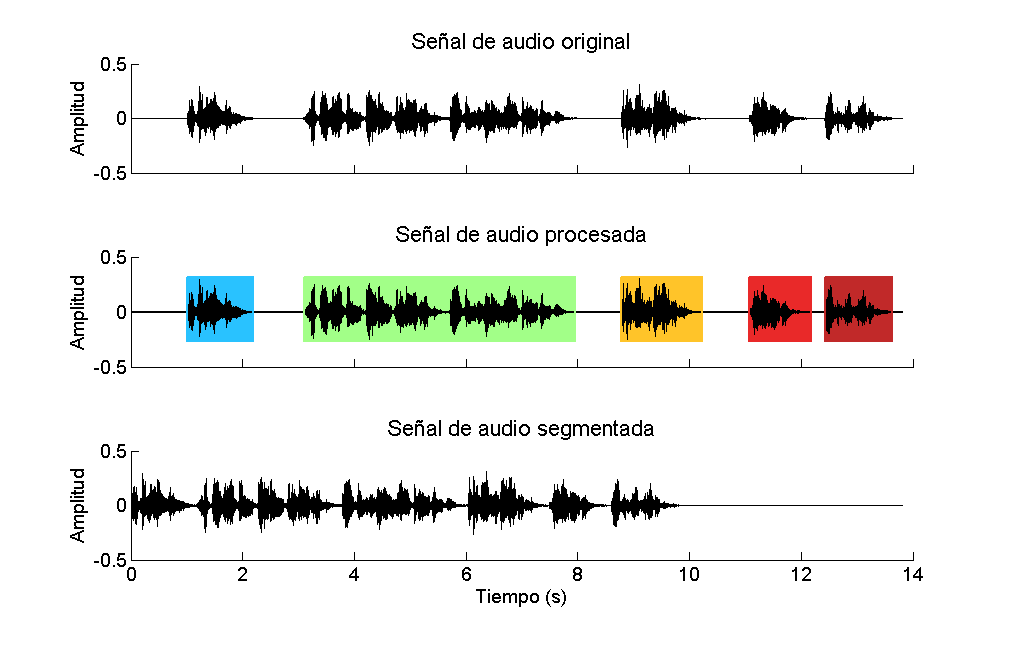
\includegraphics[width=1\textwidth]{gfx/f-silence}
  \end{center}
\end{frame}

%\subsubsection{Obtención de vector de características}

\begin{frame}{Mel Frequency Cepstrum Coefficient}
  \begin{itemize}
    \item \small{FFT (ventana) -> Banco de filtros triangular (Mel Scale) -> Log -> DCT -> MFCC}
  \end{itemize} 
  \begin{center}
    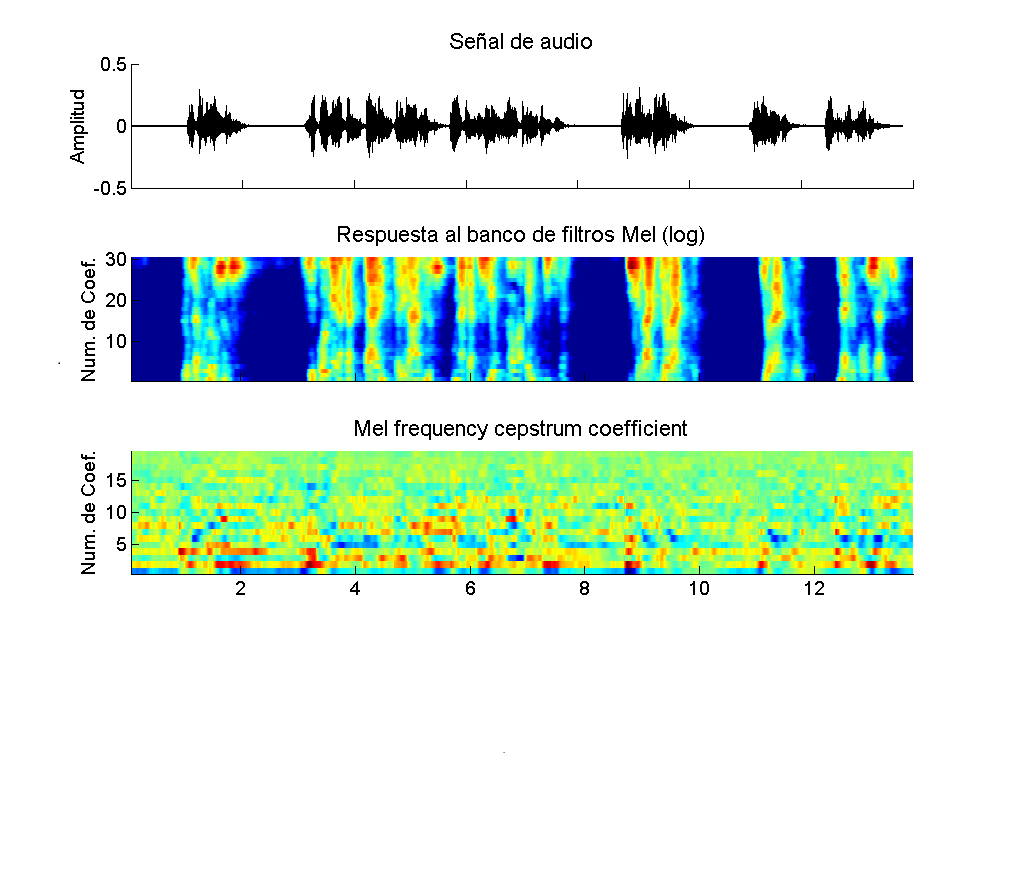
\includegraphics[width=1\textwidth]{gfx/f-mfcc}
  \end{center}
\end{frame}

%!TEX root = ../pres - final.tex

\section{Modelo}
\subsection{Hidden Markov Model}
\begin{frame}{Cadenas de Markov}
    \begin{itemize}
      \itemsep2em
      \item Cadena de Markov de primer orden      
        \\~\\
        \begin{center}
          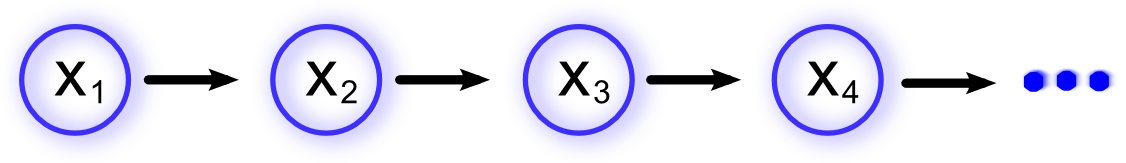
\includegraphics[width=0.4\textwidth]{gfx/mod-mm1}
        \end{center}        
        \begin{equation}
          \label{eqn:2-4}
          p(x_1, ..., x_T) 
            ~=~ \prod_{t=1}^T p(x_T ~|~ x_1, ..., x_{t-1}) 
            ~=~ p(x_1) \cdot \prod_{t=2}^T p(x_T ~|~ x_{t-1}) 
        \end{equation} 
      \item  Se puede generalizar para cadenas de Markov de un orden mayor
        \\~\\
        \begin{center}
          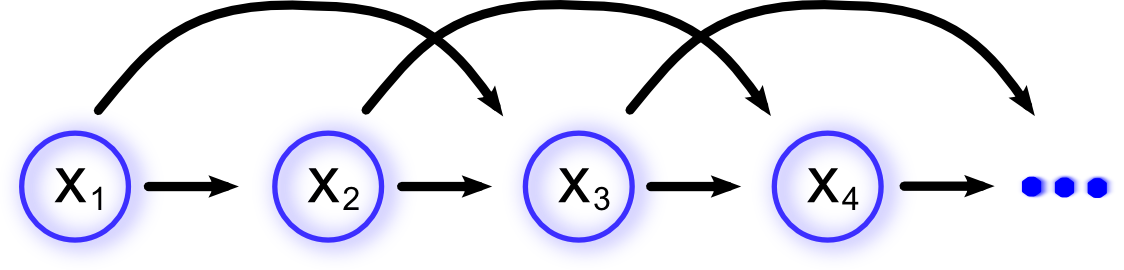
\includegraphics[width=0.45\textwidth]{gfx/mod-mm2}
        \end{center}
        \begin{equation}
          \label{eqn:2-4}
          p(x_1, ..., x_T) 
            ~=~ p(x_1) p(x_2 ~|~ x_1) \cdot \prod_{t=3}^T p(x_T ~|~ x_{t-1}, x_{t-2}) 
        \end{equation} 
  \end{itemize} 
\end{frame}

\begin{frame}{Modelo oculto de Markov}
  \begin{itemize}
    \itemsep1em
    \item Agregar una variable latente $z_t$ (discreta), que corresponda a cada observación $x_t$.
      \begin{align}
        z_{t+1} &\perp z_{t-1} ~|~ z_{t} \\
        p(x_1, ..., x_T, z_1, ..., z_T) &~=~ p(z_1) \left [ \prod_{t=2}^T p(z_t ~|~ z_{t-1}) \right ] 
          \prod_{t=1}^T p(x_t ~|~ z_{t}).
      \end{align}

    \item Modelar proceso bivariado en el tiempo. Una variable observada y una variable latente asociada.
      \\~\\
      \begin{center}
        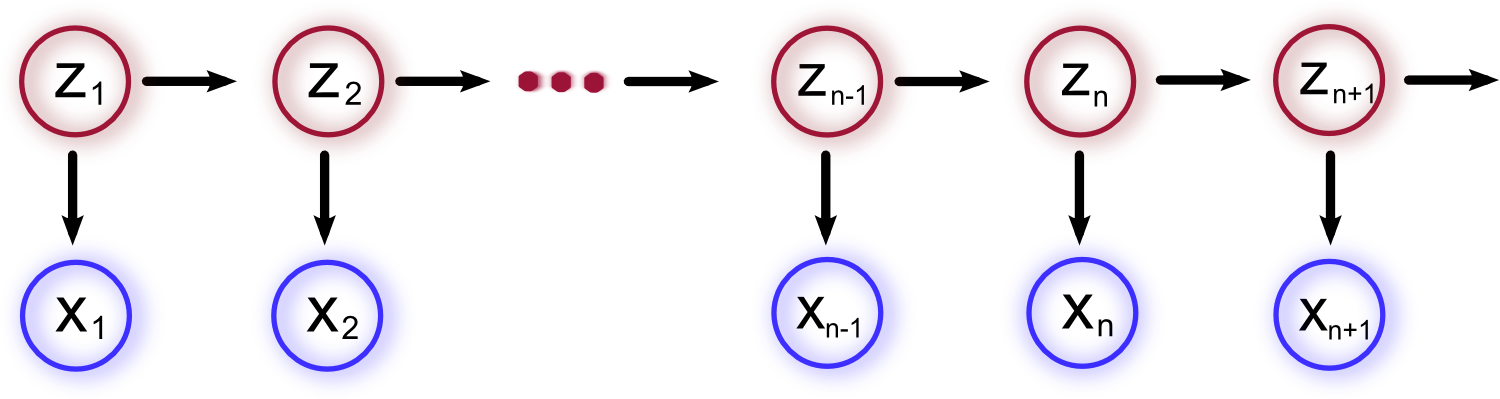
\includegraphics[width=0.5\textwidth]{gfx/mod-hmm}
      \end{center}    
      
    \item Mezcla de distribuciones en la que la densidad está dada por $p(x | z)$      
  \end{itemize}
\end{frame}

\begin{frame}{Parámetros del HMM}
  \begin{itemize}
    \item Probabilidad de cambio entre estados dada una \alert{matriz de transición} $\mathbf{A}$
      \begin{align}
        A_{jk} &\equiv p(z_{tk} = 1 ~|~  z_{t-1, j} = 1) \\
        p(z_t ~|~ z_{t-1}, \mathbf{A}) &= \prod_{k=1}^K \prod_{j=1}^K A_{jk}^{z_{{n-1}, j} \cdot z_{t,k}}
      \end{align}      
    \item \alert{Vector de distribución inicial} $\bm{\pi}$ para variable latente.
      \begin{align}
        \pi_k &\equiv p(z_{1k}) \\
        p(z_1 ~|~ \pi) &= \prod_{k=1}^K \pi_k^{z_{1k}}
      \end{align}       
    \item \alert{Probabilidad de emisión} de una variable observada $x_T$ dada una variable latente $z_T$.
      \begin{equation}
        p(x_t ~|~ z_t, \phi) = \prod_{k=1}^K p(x_T ~|~ \phi_k) ^ {z_{tk}}
      \end{equation}
  \end{itemize}
\end{frame}

\subsection{Resolver HMM con EM}

\begin{frame}{HMM con EM}
  \begin{itemize}
    \item \alert{Probabilidad conjunta del modelo}
      \begin{equation}
        p(\mathbf{X}, \mathbf{Z} ~|~ \theta)        
          = p(z_1 ~|~ \pi) \left[ \prod_{t=2}^T p(z_t ~|~ z_{t-1}, \mathbf{A}) \right]
          \prod_{t=1}^T p(x_t ~|~ z_t, \mathbf{B}, \phi)
      \end{equation}
      
      donde $\mathbf{X} = \lbrace x_1, ..., x_N \rbrace$,~ $\mathbf{Z} = \lbrace z_1, ..., z_N \rbrace$ \\~\\

      y los parámetros del modelo $\theta = \lbrace \bm{\pi}, \mathbf{A}, \mathbf{B}, \phi \rbrace$

    \item Función de verosimilitud completa
        \begin{equation}
          \mathcal{Q}(\theta, \theta^{old}) = \sum_{\mathbf{Z}} p(\mathbf{Z} ~|~ \mathbf{X}, \theta^{old})
              \log p(\mathbf{X}, \mathbf{Z} ~|~ \theta)
        \end{equation}      
  \end{itemize}
\end{frame}    

\begin{frame}{HMM con EM}
  \begin{itemize}      
      \vspace{1.5em}
      \begin{description}
        \item[Probabilidad marginal de una variable latente]
          \begin{equation}
            \gamma(z_t) &= p(z_t ~|~ \mathbf{X}, \theta^{old})
          \end{equation}

        \item[Probabilidad conjunta de dos variables latentes consecutivas]
          \begin{equation}
            \xi(z_{t-1}, z_T) &= p(z_{t-1}, z_T ~|~ \mathbf{X}, \theta^{old})
          \end{equation}
      \end{description}
  \end{itemize}
\end{frame}

\begin{frame}{HMM con EM}
  \begin{itemize}
      \item Prob. marginal de $z_{tk} = 1$, prob. conjunta de $z_{t-1,j}, z_{tk}$
        \begin{align}
          \gamma(z_{tk}) &= \mathbb{E} \left[ z_{tk} \right] = \sum_Z  \gamma(\mathbf{z}) z_{tk} \label{eq-13} \\
          \xi(z_{t-1,j}, z_{tk}) &= \mathbb{E} \left[z_{t-1, j} \cdot z_{tk} \right] = 
            \sum_Z  \gamma(\mathbf{z}) z_{t-1, j} \cdot z_{tk} \label{eq-14}
        \end{align}  
        
        \item Función de verosimilitud completa (reescrita con \eqref{eq-13}, \eqref{eq-14})
          \begin{equation}
            \begin{split}
              \mathcal{Q}(\theta, \theta^{old}) = 
              \sum_{k=1}^K \gamma(z_{1k}) \log \pi_k + 
              \sum_{t=2}^T \sum_{j=1}^K \sum_{k=1}^K \xi(z_{t-1,j}, z_{tk}) \log A_{jk} + \\
              \sum_{t=1}^T \sum_{k=1}^K \gamma(z_{tk}) \log p(x_T ~|~ \phi_k)
            \end{split}
          \end{equation}
          
         \item Parámetros estimados por EM: 
         \begin{equation}
           \pi_k = \frac{\gamma(z_{1k})}{\sum_{j=1}^K \gamma(z_1j)}, ~~
           A_{jk} = \sum_{t=2}^T \frac{\xi(z_{t-1,j}, z_{tk})}{ \sum_{l=1}^K \xi(z_{t-1,j}, z_{tl})}
         \end{equation}
  \end{itemize}
\end{frame}

\begin{frame}{Algoritmo backward-forward}
  \begin{align}
  \gamma(z_t) &= p(z_t ~|~ X) = \frac{p(X ~|~ z_t) p(z_t)}{p(X)} \\
  \gamma(z_t) &= \frac{p(x_1, ..., x_t, z_t)p(x_{t+1}, ..., x_T ~|~ z_t)}{p(X)} \\
  \gamma(z_t) &= \frac{\alpha(z_t) \beta(z_t)}{p(X)} \\  
  \end{align}
  donde 
  \begin{align}
    \alpha(z_t) &\equiv p(x_1, ..., x_t, z_t) \\
    \beta(z_t) &\equiv p(x_{t+1}, ..., x_T ~|~ z_t)  \\
    \alpha(z_t) &= p(x_t ~|~ z_t) \sum_{z_{t-1}} \alpha(z_t ~|~ z_{t-1}) \\
    \alpha(z_1) &= p(z_1) p(x_1 ~|~ z_1) = \prod_{k=1}^K \lbrace {\pi_k p(x_1 ~|~ \phi_k)} \rbrace ^ {z_{1k}}
  \end{align}  
\end{frame}

\begin{frame}{Algoritmo backward-forward}
  \begin{align}
    \beta(z_t) = \sum_{z_{t+1}} \beta(z_{t+1})p(x_{t+1} ~|~ z_{t+1}) p(z_{t+1} ~|~ z_t)
  \end{align}  
\end{frame}

\section{Bootstrap}
\begin{frame}{Bootstrap}
\end{frame}

\section{Pruebas}

\subsection{Pruebas con datos sintéticos}

\begin{frame}{Numero fijo de speakers}
\end{frame}

\begin{frame}{Numero variable de speakers}
\end{frame}

\section*{Resumen}

\begin{frame}{Resumen}
  \begin{itemize}
  \item
    The \alert{first main message} of your talk in one or two lines.
  \item
    The \alert{second main message} of your talk in one or two lines.
  \item
    Perhaps a \alert{third message}, but not more than that.
  \end{itemize}
  
  % The following outlook is optional.
  \vskip0pt plus.5fill
  \begin{itemize}
  \item
    Outlook
    \begin{itemize}
    \item
      Something you haven't solved.
    \item
      Something else you haven't solved.
    \end{itemize}
  \end{itemize}
\end{frame}

\section{Trabajo futuro}

\begin{frame}{Trabajo futuro}
\end{frame}

% All of the following is optional and typically not needed. 
\appendix
\section<presentation>*{\appendixname}
\subsection<presentation>*{Referencias}

\begin{frame}[allowframebreaks]
  \frametitle<presentation>{Referencias}
    
  \begin{thebibliography}{10}
    
  \beamertemplatebookbibitems

  \bibitem{Author1990}
    A.~Author.
    \newblock {\em Handbook of Everything}.
    \newblock Some Press, 1990.
 
    
  \beamertemplatearticlebibitems

  \bibitem{Someone2000}
    S.~Someone.
    \newblock On this and that.
    \newblock {\em Journal of This and That}, 2(1):50--100,
    2000.
  \end{thebibliography}
\end{frame}

\end{document}